%!TeX root=../tese.tex

\chapter{Experiments and results}
\label{cap:experiments}

To understand the performance of the algorithm in practice, we proposed two experiments: one tries to identify phase transition behavior in the solution, and the other analyses its empirical run time complexity.

\section{Phase transition analysis}
\label{sec:phase-trans}

The phenomenon of \emph{phase transition} was conjectured as a property of all NP-complete problems \citep{cheeseman1991really} and was further studied for PSAT problems \citep{Finger2011ProbabilisticSL}. In the last study, experiments were made by the rate $m/n$, where $m$ is the number of 3-SAT clauses and $n$ is the number of variables; also, it was used $k$ fixed probability assignments to uniformly distributed random PSAT instances. Then, it was shown that, when $m/n$ is small, almost all instances are satisfied and, when $m/n$ is high, instances are unsatisfiable; this is called \emph{first-order phase transition}. Also, for NP-Complete problems, harder instances concentrate between satisfiability and unsatisfiability; and this is called \emph{second-order phase transition}.

Based on the work of \citeauthor{Finger2011ProbabilisticSL}, we create a similar experiment for $\pgelsat$, with randomly generated $\pgel$-KBs. Consider a probabilistic KB with $n$ concepts, $n_R$ roles, $m$ concept inclusions in the normal form, and $p$ uncertain axioms with $p$ probabilistic restrictions of the form $P(C \isa D) \leq b$, where $b \in \Ratios$ and $C, D$ are concepts. For this experiment, fix $n$, $n_R$, $p$ and vary $m$. For each value of $m$, generate several instances of $\pgel$-KBs as a random graph with linear restrictions.

The random KB generation is described as follows. Start with a graph $G$ with no edges and 3 vertices: $\bot, \top$ and $Init$; add $n$ vertices and $n_R$ roles to $G$. Then, add $m$ edges correspoding to certain axioms, and $p$ edges correspoding to uncertain axioms. Edges are added by choosing randomly two vertices $C$ and $D$ ($n+3$ possibilities for each one), their role is chosen uniformly from $C \isa D$ and the $n_R$ other roles ($C \isa \exists r_i.D$). Also, a probabilistic restriction of the form $P(C \isa D) \leq b$ is generated for each uncertain axiom $C \isa D$, with a uniformly random $b \in [0, 2]$.

For this experiment, we fixed $n = 700$, $n_R = 3$, $p = 10$ and increased $m$ from $100$ to $2000$ in steps of $10$. For each value of $m$ we generated $500$ instances of $\pgelsat$, computed the ratio of satisfiable instances (\%$\pgelsat$) and average run time. Also, it is applied a simple moving average with an window of 5 points to the curve.  Then, we obtained the graphic in the \autoref{fig:plot-phase}.

\begin{figure}[ht]
  \centering
  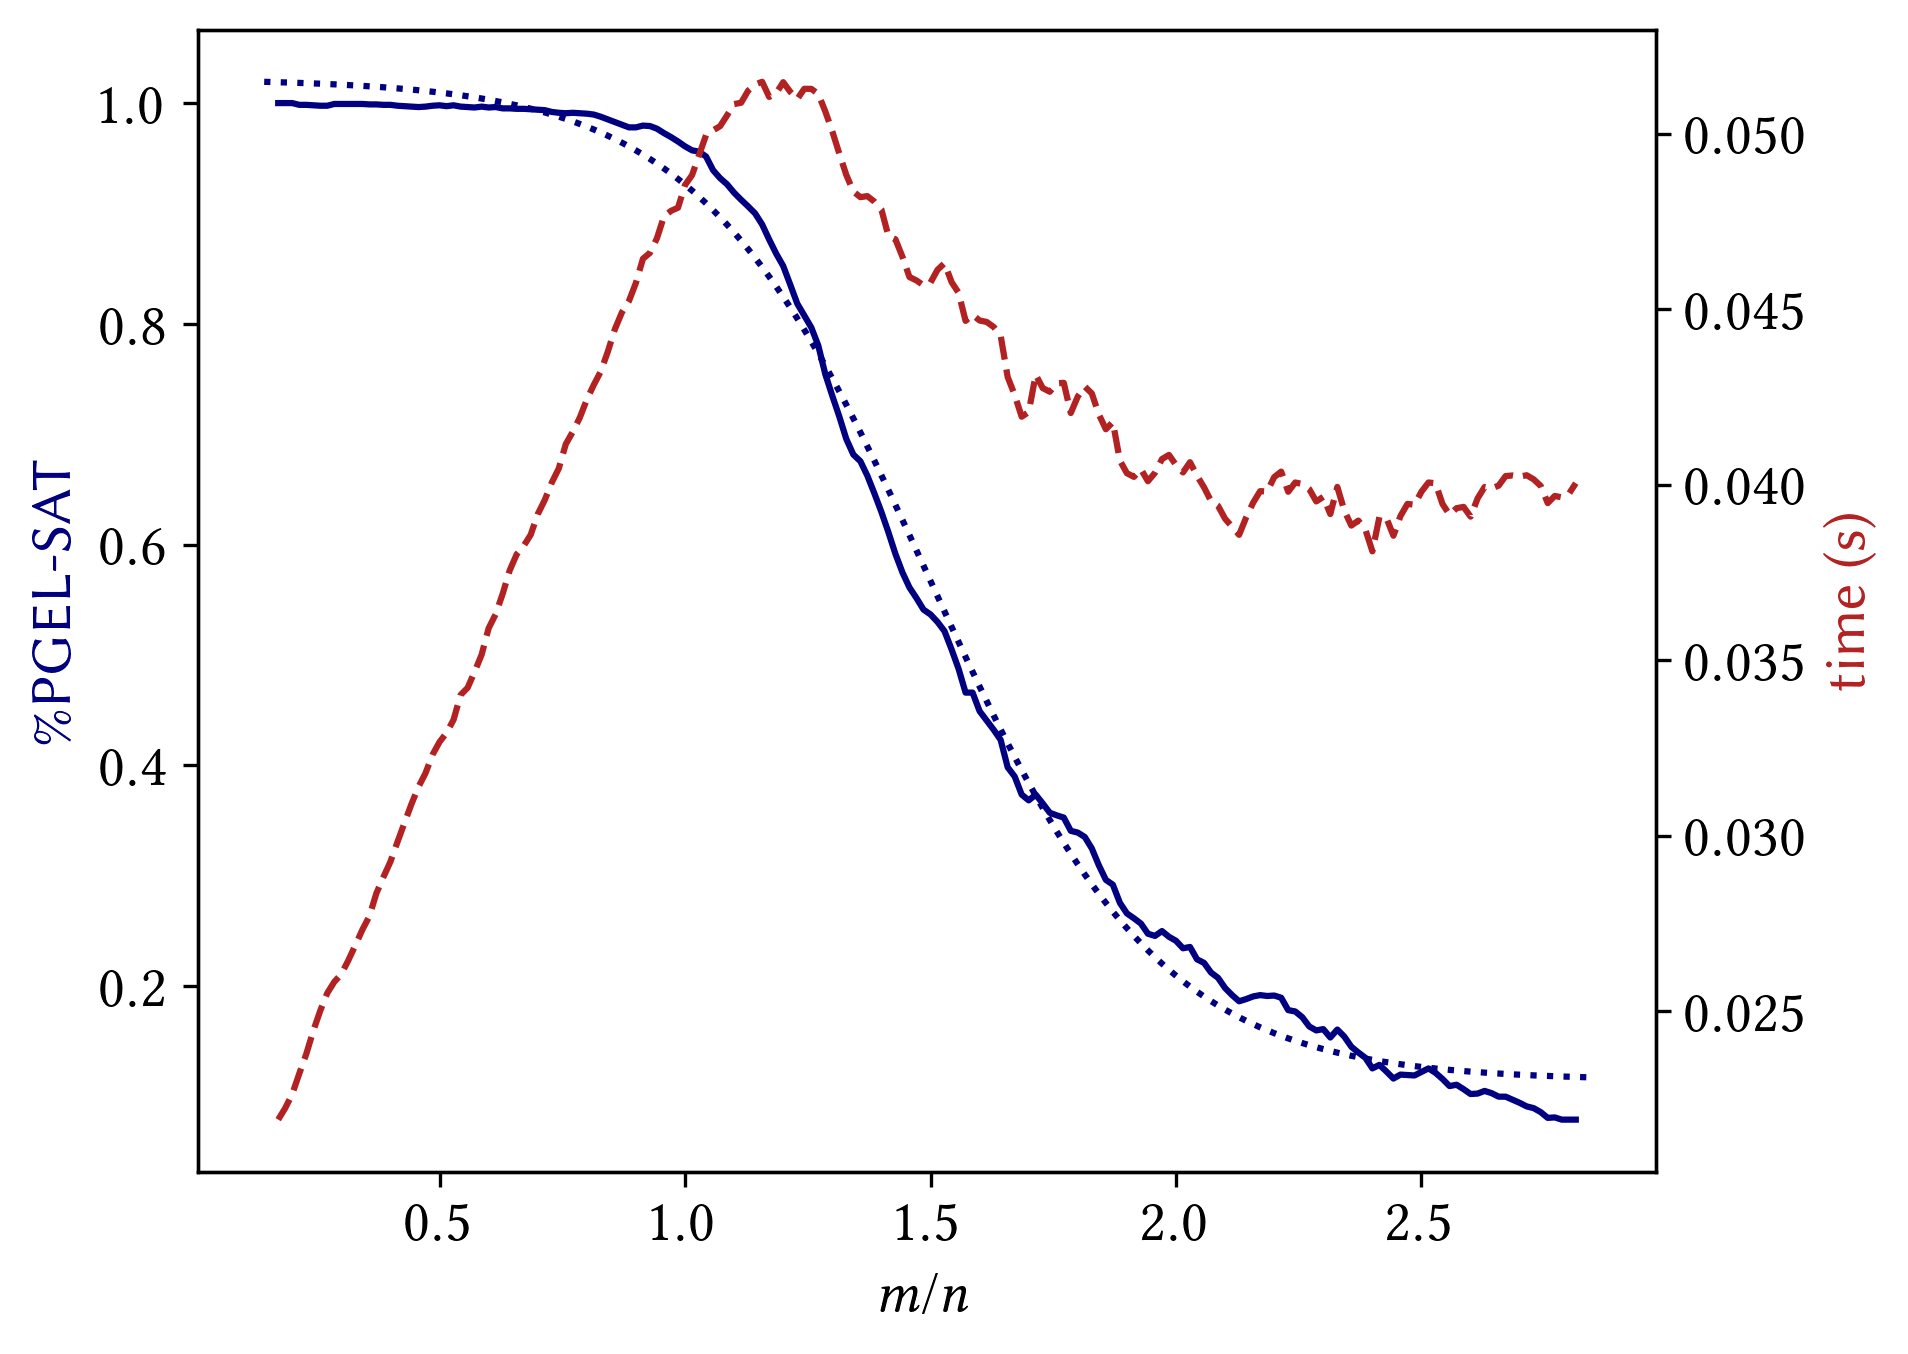
\includegraphics[width=.75\textwidth]{../img/plot-phase-trans}
  \caption{\%-satisfiable of $\pgelsat$ and average run time for instances of formulas in several cases}
  \label{fig:plot-phase}
\end{figure}
  

These experiments show that:
\begin{enumerate}[label=(\alph*)]
	\item There is an S-shaped first-order phase transition, from mostly satisfiable to mostly unsatisfiable, like its propositional problem;
	\item There is not a second-order phase transition, which is usually characterized by a high peak when satisfiability ratio is in $0.5$. We can see that, when $m/n$ increases, the average time increases until the ratio of satisfiability starts to decrease. This can be explained because the algorithm tries to find an inconsistency. Consequently, when the axioms or restrictions are higher, it is easier to find such inconsistency.
\end{enumerate}

\section{Run time analysis}

This experiment aims to estimate empirically the time complexity of the algorithm and verify its tractability.

Consider a probabilistic KB as defined in \autoref{sec:phase-trans}. Create three experiments for each parameter $n, m$ and $p$; varying one parameter and fixing others. For each value of the varying parameter, generate several instances of $\pgel$-KBs as described in \autoref{sec:phase-trans}.

For this experiment, the fixed parameters had the values $n = 10, n_R = 3, m = 10$ and $p = 10$. Each parameter $n, m$ and $m$ varied from $10$ to $400$ in steps of $20$. For each varying value, we generated $100$ instances of $\pgelsat$, computed the average run time, average run time of a single iteration and number of iterations. Also, it is applied a simple moving average with an window of 5 points to the curves.  Then, we obtained the graphics in \autoref{fig:plot-comp-1}, \autoref{fig:plot-comp-2} and \autoref{fig:plot-comp-3}. 

These experiments show that:
\begin{enumerate}[label=(\alph*)]
  \item The increase of axioms and concepts has low impact in the run time and the number of iterations;
  \item The increase of uncertain axioms has high impact in the run time;
  \item The number of iterations increases linearly with the number of uncertain axioms.
\end{enumerate}
Then, we have a result similar to the estimated complexity in \autoref{sec:time-compl}.

However, one could argue that the run time growth of varying uncertain axioms is exponential. Thus, we propose a new experiment to analyse this curve.

Using the same data from the previous experiment, we applied the Levenberg–Marquardt algorithm \citep{levenberg1944method,marquardt1963algorithm}, which is a method for solving non-linear least squares problems. This method was applied with the SciPy's implemention called \textsf{curve\_fit} \citep{2020SciPy-NMeth}. 

Define a polinomial $p(x)$ and an exponential function $e(x)$, such that
\begin{align*}
  p(x) &:= A_7 \cdot x^7 + A_6 \cdot x^6 + A_5 \cdot x^5 +A_4 \cdot x^4 + A_3 \cdot x^3 + A_2 \cdot x^2 + A_1 \cdot x + A_0\\
  e(x) &:= B_2 \cdot 2^{B_2 \cdot x} + B_0.
\end{align*}
We want to find parameters $A_0, \dots, A_7$ and $B_0, \dots, B_2$ in such a way that $p(x)$ and $e(x)$ best approximate the experimental measures. 

After applying the algorithm, we obtain $p(x)$ and $e(x)$ with the following approximated parameters, which are illustrated in the \autoref{fig:plot-comp-prob},
\begin{align*}
  p(x) :=& -1.5  \cdot  10^{-15} \cdot x^7 
        + 2 \cdot 10^{-12} \cdot x^6 
        - 1 \cdot 10^{-9} \cdot x^5 
        + 2.9 \cdot 10^{-7} \cdot x^4\\ 
        &- 4 \cdot 10^{-5} \cdot x^3 
        + 2.8  \cdot  10^{-3}\cdot x^2 
        - 0.08 \cdot x 
        + 0.64\\
  e(x) :=& \, 0.282 \cdot 2^{0.014 \cdot x} - 0.592.
\end{align*}
From this analysis, we have that:
\begin{enumerate}[label=(\alph*)]
  \item The terms that mostly contribute to the growth of $p(x)$ have a small degree ($x^4$ and $x^2$);
  \item The factor multipling $x$ in $e(x)$ is small ($\approx 0.014$); therefore, $e(x)$ corresponds to the function $f(x) = 0.282 \cdot (1.01)^{x} - 0.592$, which has a very small exponential growth rate.
\end{enumerate}
Thus, there is no experimental results to refute that the run time growth of \textsc{PGEL-SAT-Solver} is not polynomial. 

\begin{figure}[ht]
  \centering
  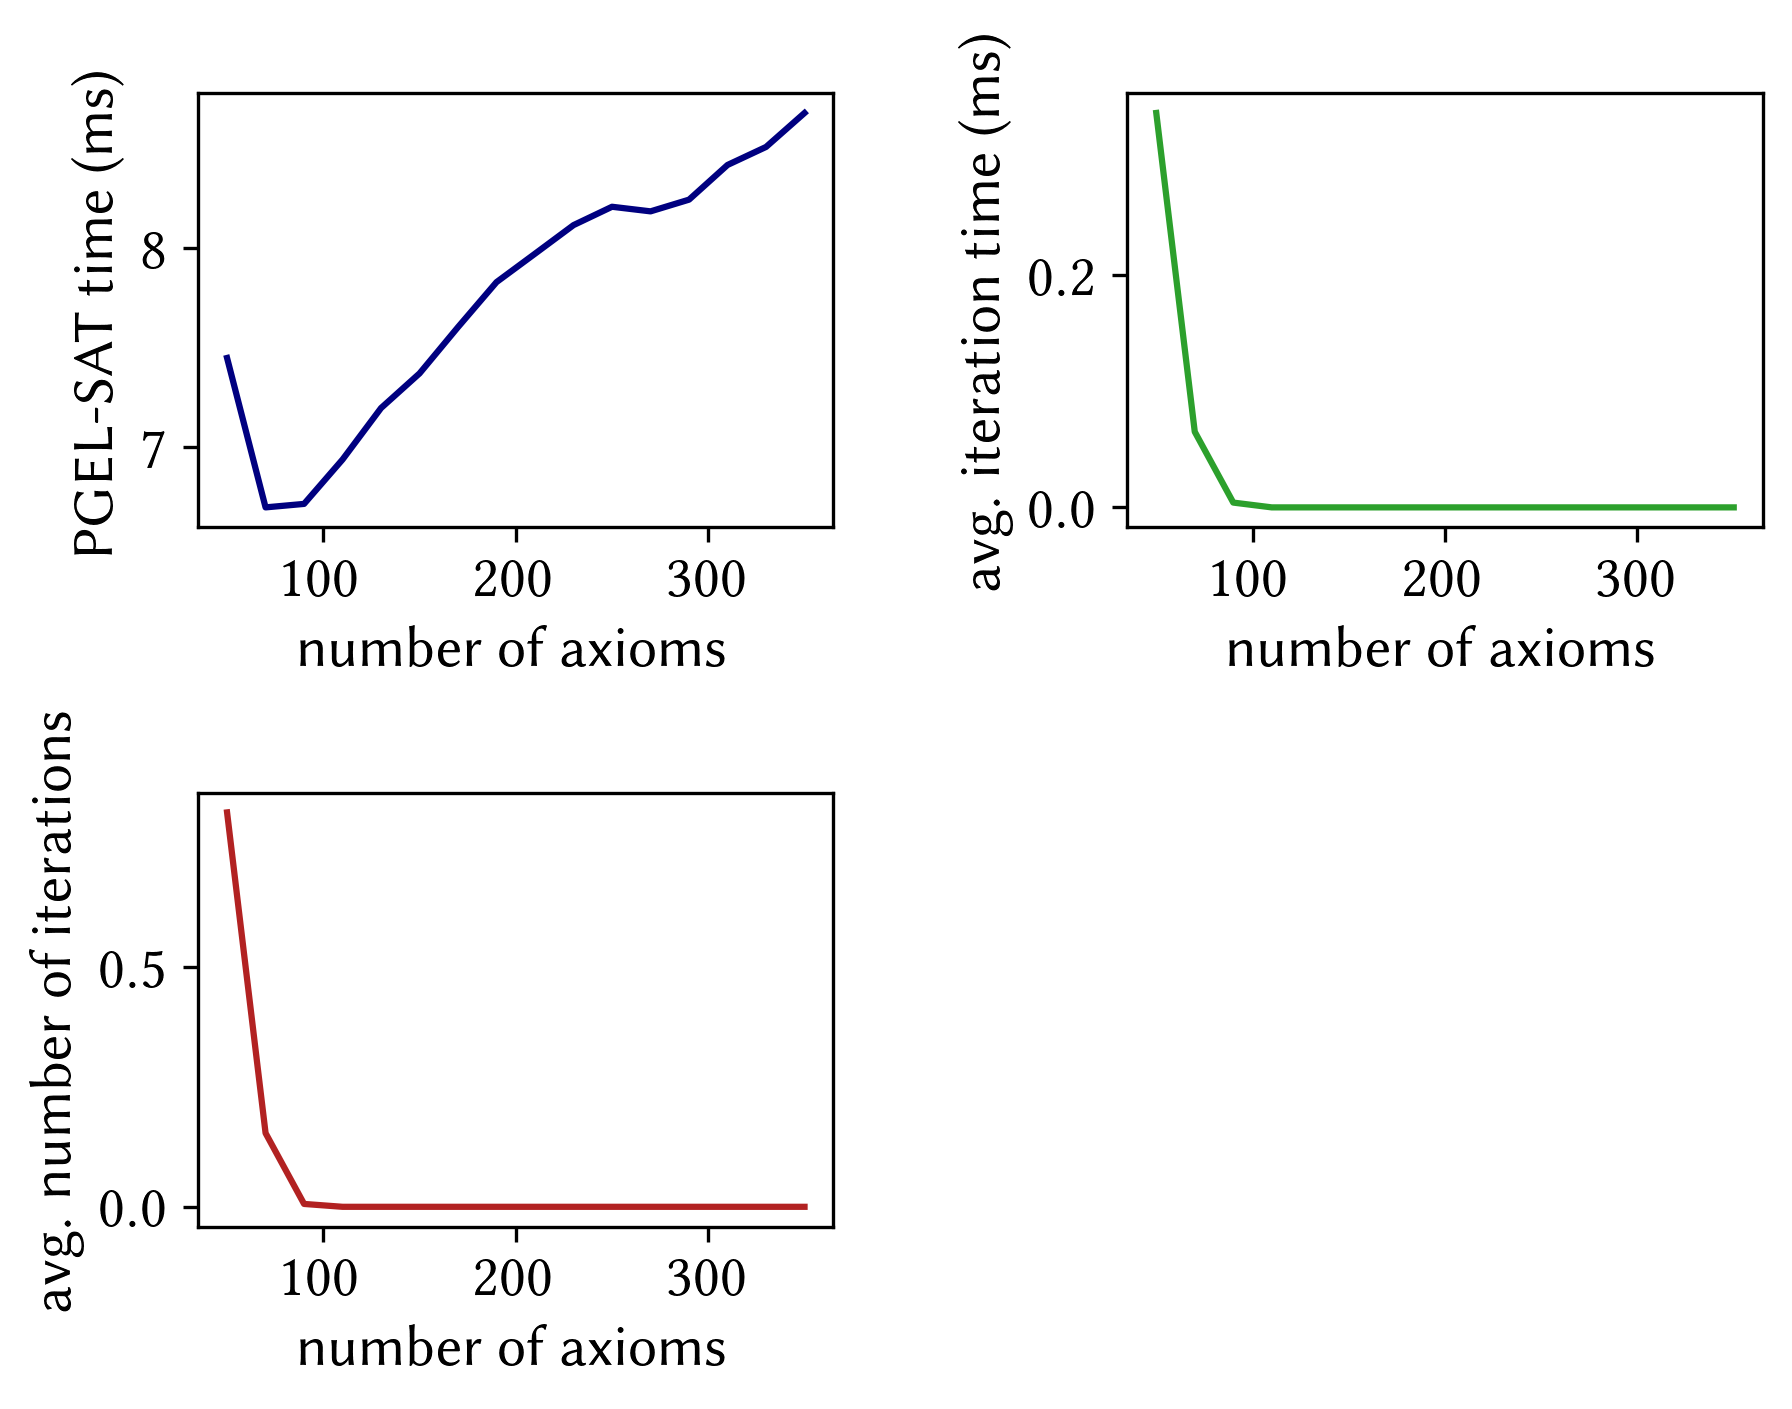
\includegraphics[width=.75\textwidth]{../img/plot-comp1-0}
  \caption{Impact of the increase of certain axioms in the run time and number of iterations}
  \label{fig:plot-comp-1}
\end{figure}

\begin{figure}[ht]
  \centering
  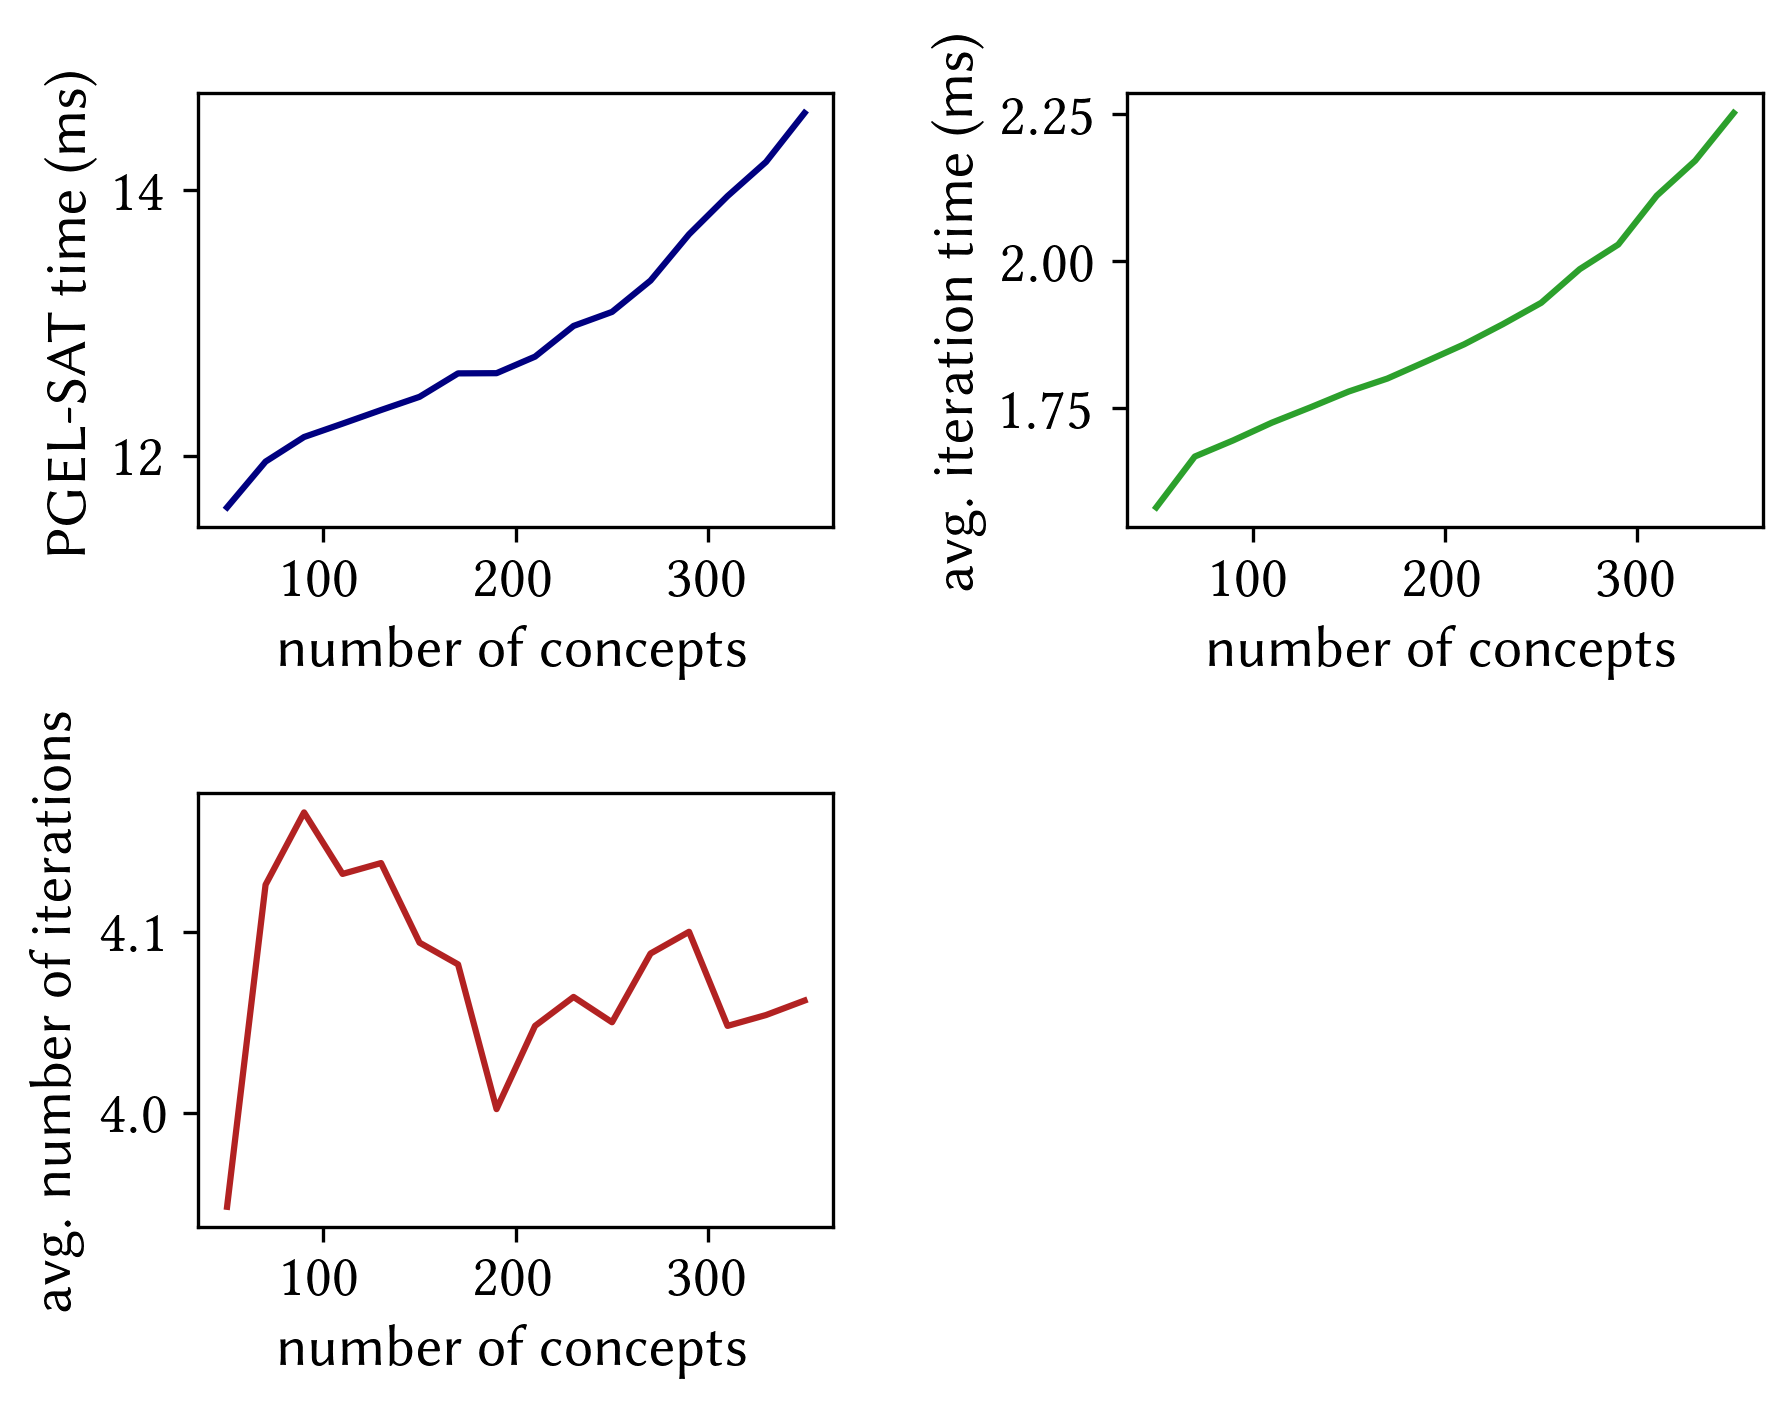
\includegraphics[width=.75\textwidth]{../img/plot-comp1-1}
  \caption{Impact of the increase of concepts in the run time and number of iterations}
  \label{fig:plot-comp-2}
\end{figure}

\begin{figure}[ht]
  \centering
  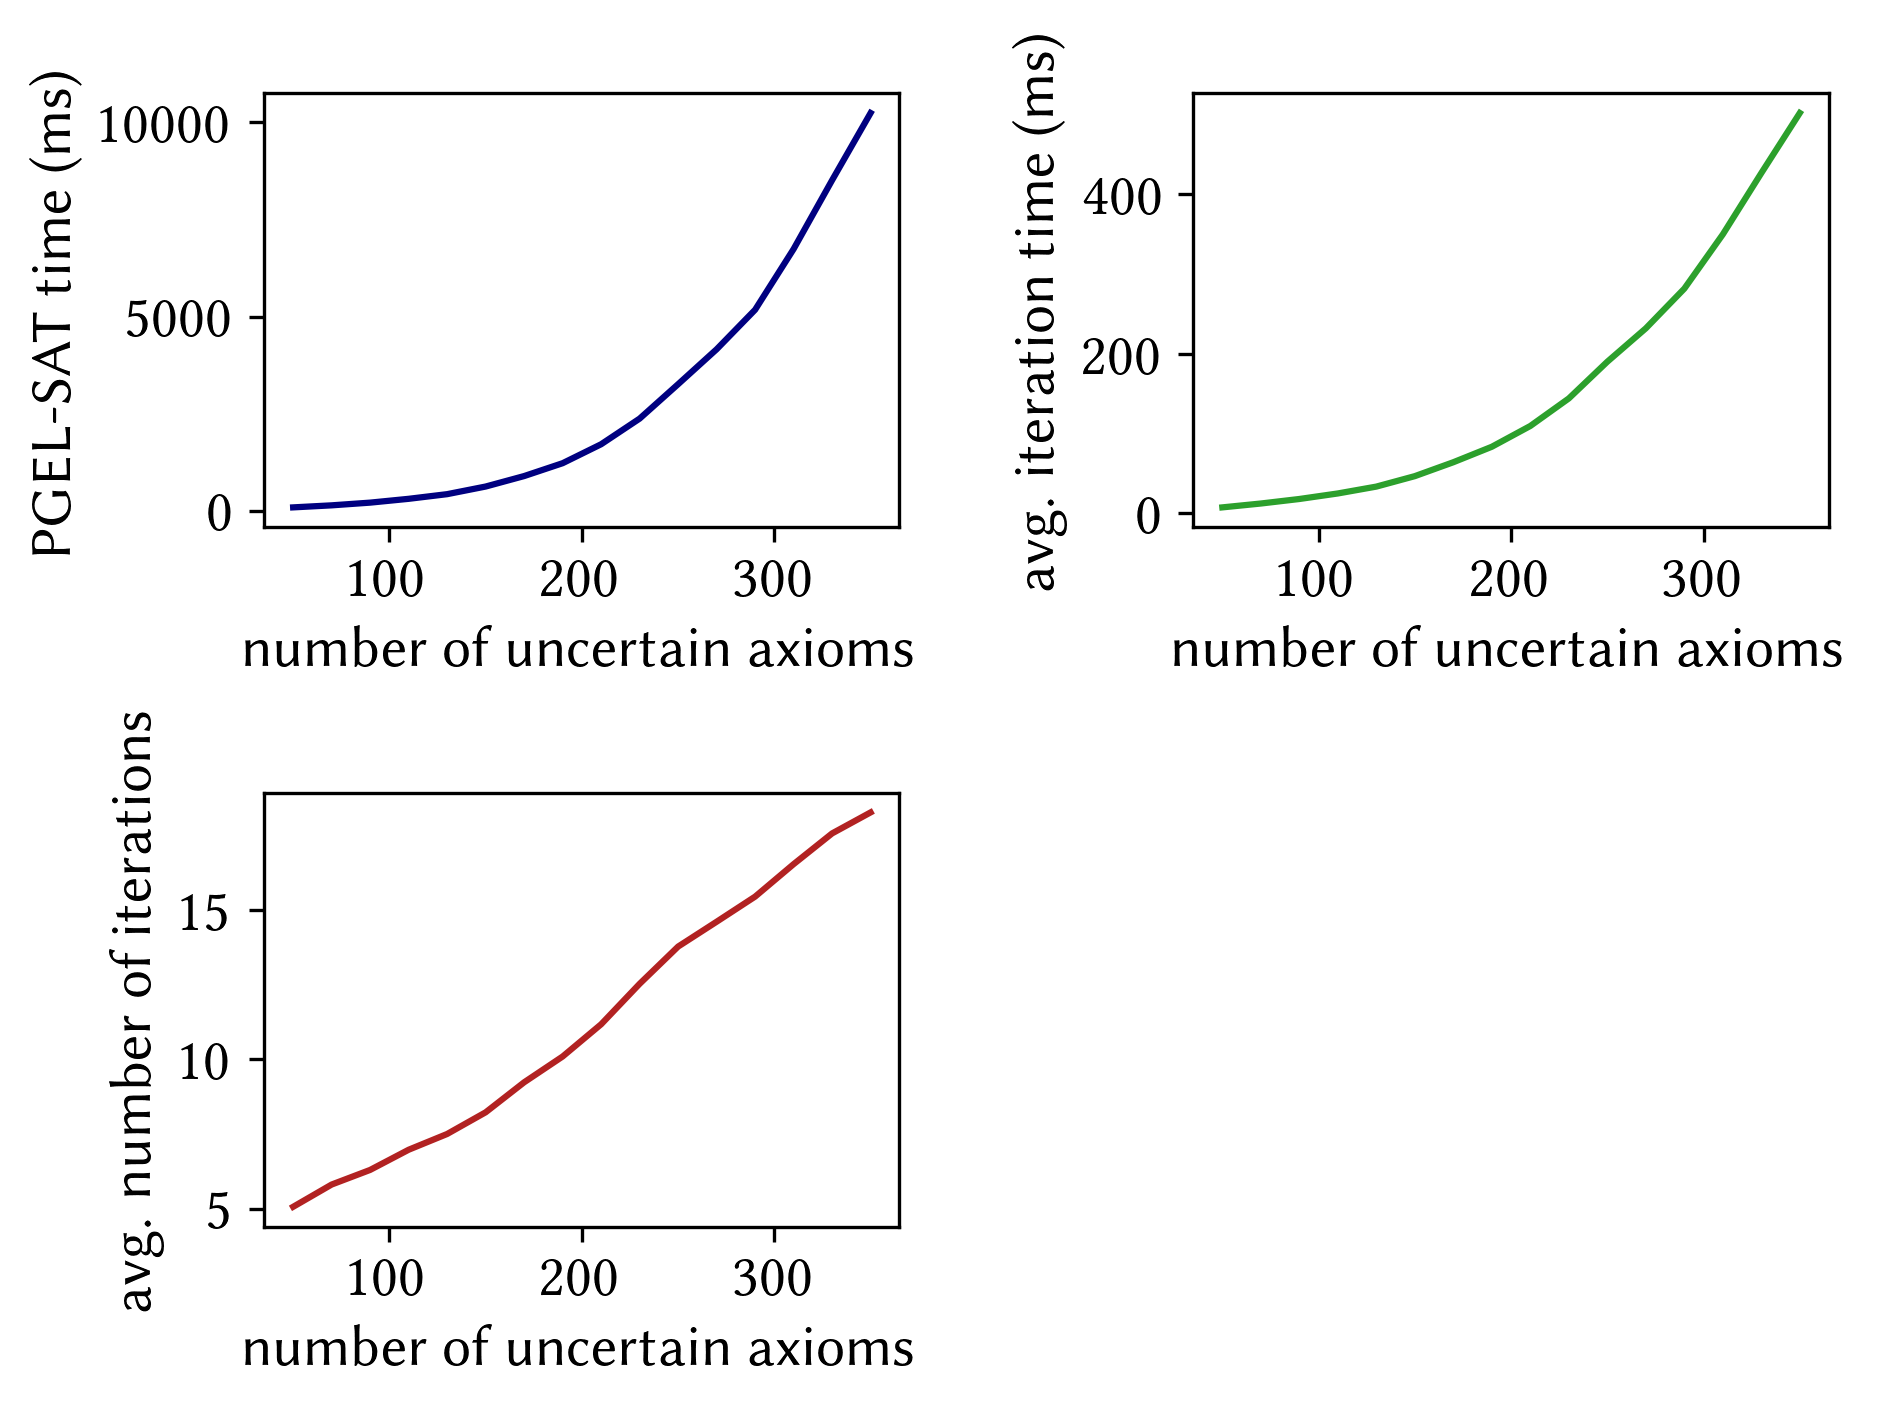
\includegraphics[width=.75\textwidth]{../img/plot-comp1-2}
  \caption{Impact of the increase of uncertain axioms in the run time and number of iterations}
  \label{fig:plot-comp-3}
\end{figure}

\begin{figure}[ht]
  \centering
  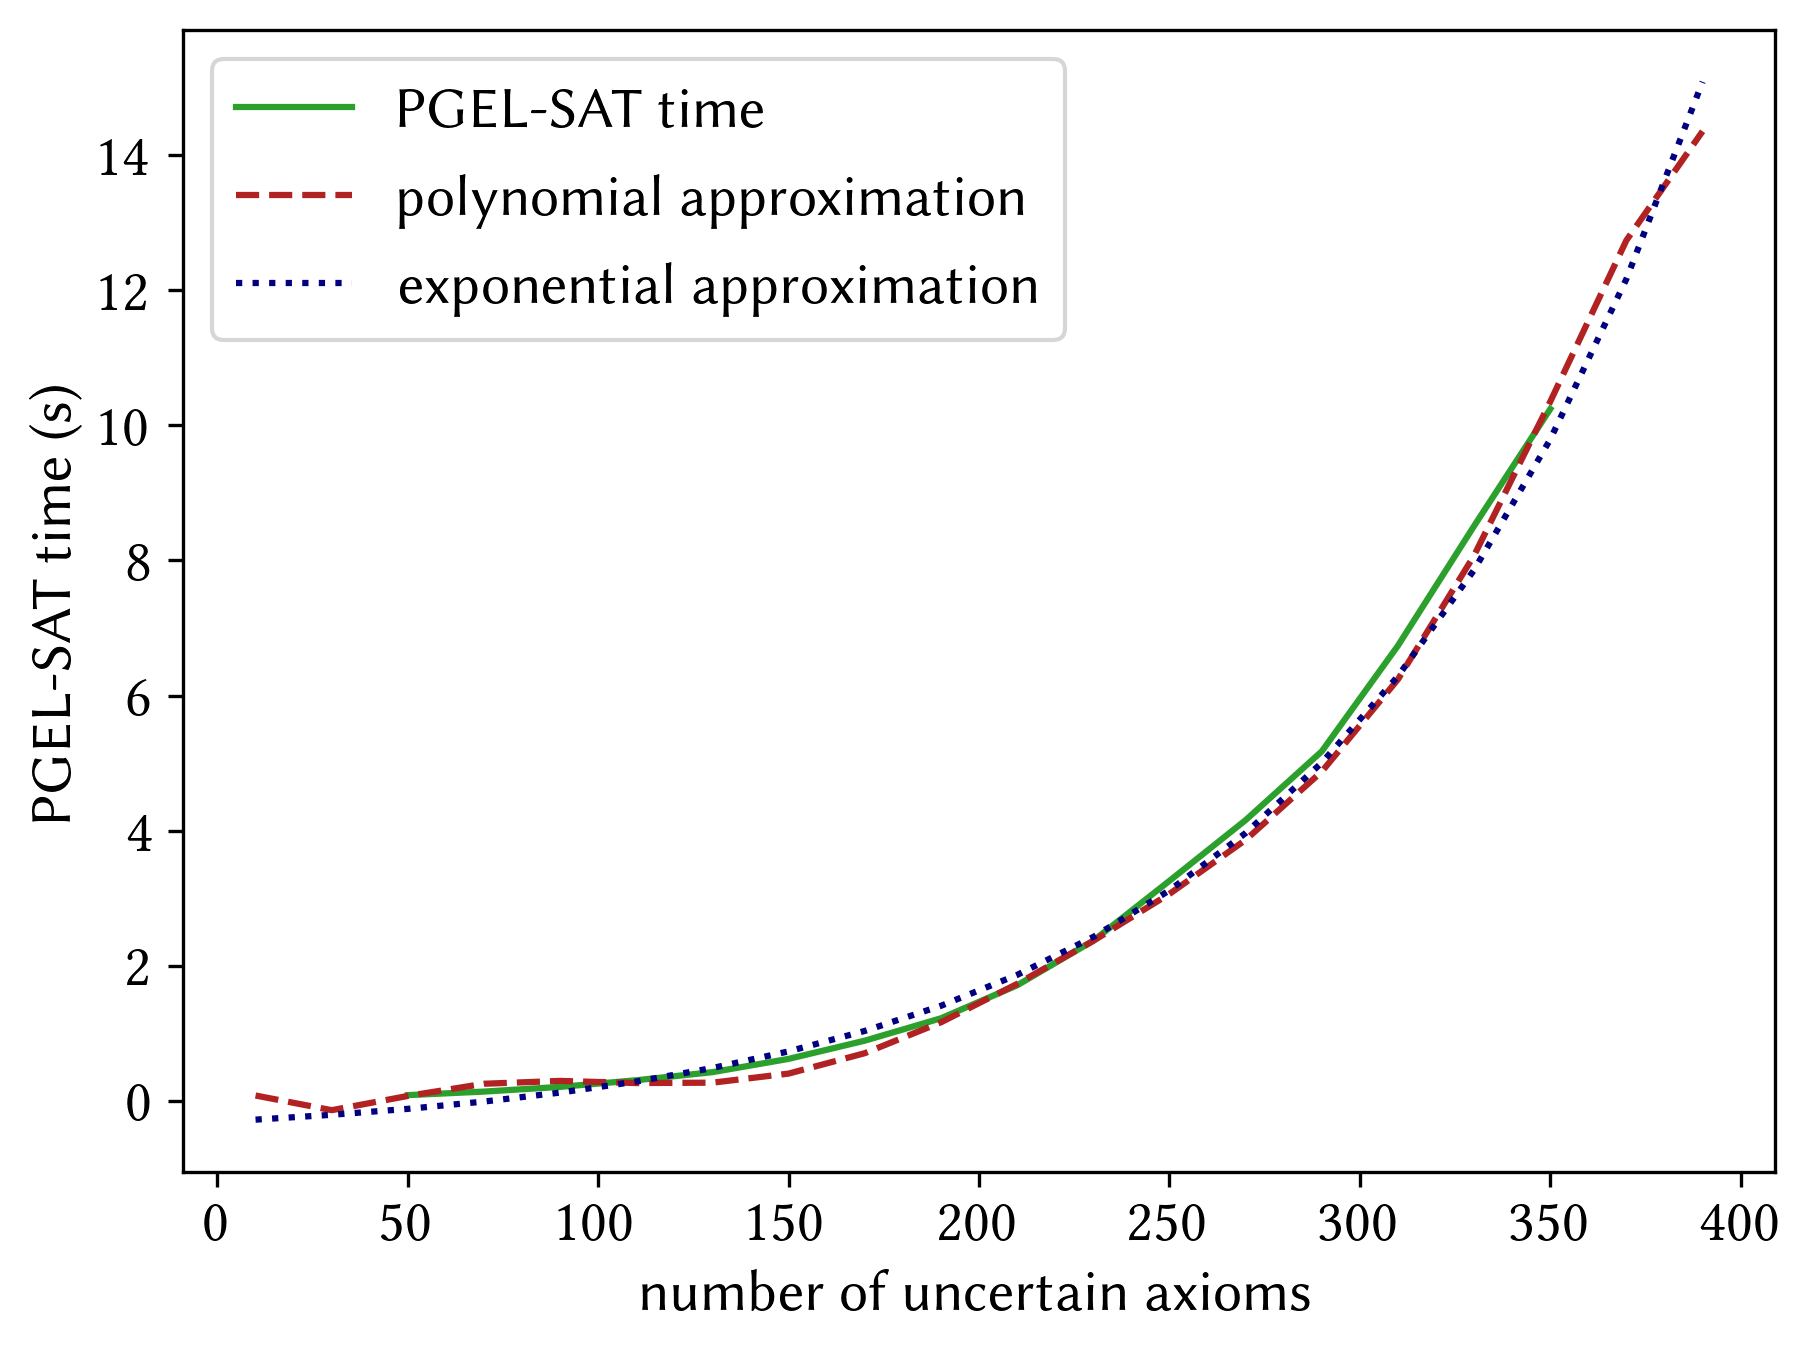
\includegraphics[width=.75\textwidth]{../img/plot-comp2}
  \caption{Polynomial and exponential approximations of the run time growth by varying the number of uncertain axioms}
  \label{fig:plot-comp-prob}
\end{figure}

As expected, these algorithms do not have the phase transition behavior of NP-Complete problems and do not show any exponential run time growth rate. Then, these initial experiments confirm that \textsc{PGEL-SAT-Solver} is a promising algorithm for tractable probabilistic reasoning over description logics.
